\chapter{Knowledge Graph\protect\footnote{Part of the Python code for this section was adopted from \cite{projdigi}}}\label{ch:knowledge_graph}
\section{Introduction}
As outlined in Chapter \ref{ch:introduction}, the goal of this project was to extract structured information from unstructured text and store this information in a Knowledge Graph.
A Knowledge Graph is an organized representation of real-world entities and their relationships which is typically stored in a graph database such as neo4j \cite{neo4j-kgdefinition}.
A graph database stores data as \emph{Nodes}, \emph{Relationships} and \emph{Properties} in a graph-like \cite{graph-definition} structure instead of in tables or documents \cite{neo4j}.
This enables the database to traverse \emph{Nodes} and \emph{Relationships} more quickly than relational databases, that would use computationally expensive \emph{JOIN} operations to retrieve inter-related information \cite{neo4j-kgdefinition}.

All the files for this chapter can be found in the \emph{src/F\_knowledge\_graph} directory.

\section{Knowledge Graph Creation}
A Knowledge Graph is defined by an \emph{Organizing Principle} \cite{neo4j-kgdefinition} or a \emph{Schema}.
The schema of the Knowledge Graph in this project is depicted in Figure \ref{fig:kg-schema-2}.
\begin{figure}[H]
	\centering
	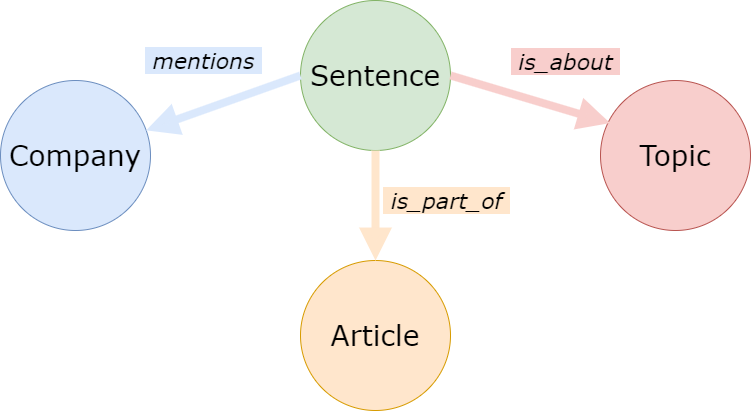
\includegraphics[width=0.75\textwidth]{Assets/kg_schema}
	\caption{Knowledge Graph Schema}
	\label{fig:kg-schema-2}
\end{figure}
The schema contains four Nodes (\emph{Article}, \emph{Sentence}, \emph{Company}, \emph{Topic}) and
three relationships (\emph{mentions}, \emph{is\_part\_of}, \emph{is\_about}), as described in Section \ref{ch:introduction}.

\paragraph{Ontology}
A Knowledge Graph \emph{Schema} can be outlined in different ways, for instance by using an \emph{Ontology}.
An \emph{Ontology} uses a modelling language to formally specify the concepts and relationships in a human- and machine-understandable way \cite{neo4j-kgdefinition}.

The most widely used ontology modelling languages are OWL (\emph{Web Ontology Language}) \cite{owl} and RDFS (\emph{Resource Description Framework Schema}) \cite{rdfs}.
Their most fundamental construct is a triple \cite{triples} consisting of
\begin{center}
\textbf{Subject - Predicate - Object}
\end{center}
tuples.
Multiple triples can be composed into a graph structure because objects can be subjects and vice versa and both can be connected via predicate relationships.\\
The textual presentation of the Ontology in this project is done with a Turtle \cite{turtle} file (suffix: \emph{.ttl}), a common data serialization format for storing triples.
The \emph{NewsArticles.ttl} Ontology file (Python-Code \ref{code:onto1}-\ref{code:onto3}) was created with Protege \cite{protege}, an open-source ontology editor by Stanford University.

\begin{listing}[H]
    \captionof{listing}{NewsArticles.ttl - Prefixes}
    \inputminted[
    firstline=1,
    lastline=8,
    firstnumber=1,
    ]{python}{/media/rainergo/PROJECTS/UASFRA-MS-Thesis/src/F_knowledge_graph/Ontologies/NewsArticles.ttl}
    \label{code:onto1}
\end{listing}

Turtle files usually start with prefixes that refer to other Ontology namespaces \cite{owl-guide} and their vocabulary \cite{owl-guide}.

In line 8 of the \emph{NewsArticles.ttl} file, the triple
\begin{center}
    \emph{subject}  ~~~~~~~~~~    \emph{predicate}  ~~~~~~~~~~  \emph{object}\\
    \textbf{rainergo: ~~~~~ rdf:type ~~~~~ owl:Ontology}
\end{center}
states that the prefix \emph{rainergo} in line 1 is of type \emph{Ontology} where \emph{type} and \emph{Ontology} themselves
are defined in triples that are accessible through their public \glspl{iri} in lines 2 and 3.

\begin{listing}[H]
    \captionof{listing}{NewsArticles.ttl - Classes or Nodes}
    \inputminted[
    firstline=87,
    lastline=101,
    firstnumber=87,
    ]{python}{/media/rainergo/PROJECTS/UASFRA-MS-Thesis/src/F_knowledge_graph/Ontologies/NewsArticles.ttl}
    \label{code:onto2}
\end{listing}

In lines 87 to 101, the classes or Nodes of the Knowledge Graph schema are defined, again with triples.

\begin{listing}[H]
    \captionof{listing}{NewsArticles.ttl - Relationships}
    \inputminted[
    firstline=10,
    lastline=27,
    firstnumber=10,
    ]{python}{/media/rainergo/PROJECTS/UASFRA-MS-Thesis/src/F_knowledge_graph/Ontologies/NewsArticles.ttl}
    \label{code:onto3}
\end{listing}

In lines 10 to 27, the relationships are defined with three triples for each relationship
where the second (predicate: \emph{domain}) and third (predicate: \emph{range}) triple represent its source and target Node.

\begin{listing}[H]
    \captionof{listing}{NewsArticles.ttl - Properties}
    \inputminted[
    firstline=29,
    lastline=50,
    firstnumber=29,
    ]{python}{/media/rainergo/PROJECTS/UASFRA-MS-Thesis/src/F_knowledge_graph/Ontologies/NewsArticles.ttl}
    \label{code:onto4}
\end{listing}

In Python Code \ref{code:onto4}, lastly the Node's properties and their data types are defined (only shown for the Node type \emph{Article}).\\

The Turtle file represents the human- and machine-readable presentation of the Schema that in Figure \ref{fig:kg-schema-2} was visualized as chart.

\paragraph{Graph Preparation}\label{par:graph-prep}
To translate the Ontology into a neo4j schema and lay the foundation for the Knowledge Graph,
the Python library \emph{rdflib} \cite{rdflib} was used in the
\begin{center}
\emph{F\_knowledge\_graph/A\_rdf\_graph.py}
\end{center}
module.
The functions in the \emph{RDFGraph} class parse the triples in the \emph{NewsArticles.ttl} file into an RDF \cite{rdfs} graph and construct \gls{cypher} \cite{cypher} query templates based on this graph for subsequent data imports.
\gls{cypher} \cite{cypher} is a declarative graph query language whose query commands are similar to those of the popular SQL \cite{sql} database language used for relational databases.\\

The functions to operate on the neo4j graph database and to run \gls{cypher} queries can be found in the
\begin{center}
    \emph{F\_knowledge\_graph/B\_graph\_construction}
\end{center}
module within the \emph{GraphConstruction} class.
They require the neo4j database and the neo4j Python driver to be installed \cite{neo4j}.

\paragraph{Data Preparation}
In order to align the Knowledge Graph schema (Fig.\ref{fig:kg-schema-2}) with the extracted data in the pandas DataFrame and insert the data into the Knowledge Graph, some data preparation is necessary.

For the Topic Modelling task, the pandas DataFrame must contain one row for each sentence to be topic-classified and this was achieved by the
\begin{center}
\emph{convert\_nested\_ner\_coref\_dict()} function (Python-Code \ref{code:unnest-dict-after-coref-and-ner})
\end{center}
as outlined in Section \ref{par:topic-sents}.
But each sentence might contain multiple company references as shown in Python-Code \ref{code:dict-after-coref-and-ner-2}
where two companies, \emph{Hypoport SE} and \emph{JDC Group AG}, are mentioned in one sentence:

\begin{listing}[H]
    \captionof{listing}{Company information for each sentence}
    \inputminted[
    firstline=1,
    lastline=24,
    firstnumber=1,
    fontsize=\tiny,
    ]{python}{/media/rainergo/PROJECTS/UASFRA-MS-Thesis/doc/Assets/after_ner_coref.json}
    \label{code:dict-after-coref-and-ner-2}
\end{listing}

To prepare the DataFrame for the Knowledge Graph, the information in the Python list of dictionaries (line 4-20 in Python-Code \ref{code:dict-after-coref-and-ner-2}) must be further resolved so that each DataFrame row only contains one company mention.\\
This is what the function \emph{prepare\_df\_for\_kg()} in the \emph{main\_process.py} file does:

\begin{listing}[H]
    \captionof{listing}{Function: prepare\_df\_for\_kg()}
    \inputminted[
    firstline=91,
    lastline=100,
    firstnumber=91,
    ]{python}{/media/rainergo/PROJECTS/UASFRA-MS-Thesis/main_process.py}
    \label{code:prepare-for-kg}
\end{listing}

It extracts and inserts the \emph{entities} list into the new DataFrame column \emph{ner\_coref\_entities} (line 92),
inserts new rows that accommodate each company information separately (line 93) and therefrom extracts and pastes the \emph{comp\_symbol} and \emph{comp\_name} into new columns (line 94-95).
There are also news articles in the DataFrame that are only updates of previous articles and in which only a few words might have changed.
It is therefore possible, that same sentences appear in more than one DataFrame row, i.e. that there are duplicates which must be removed (line 97).

\paragraph{Company Symbol and \gls{isin}}\label{par:symbol-isin}
The \emph{comp\_symbol} refers to the stock ticker symbol that a company has on a certain stock exchange.
Unfortunately, these ticker symbols without their country suffixes are unique only within each stock exchange but not across stock exchanges.
\glspl{isin} on the other side are unique but unfortunately are not provided by the company data provider OpenBB \cite{openbb}.

Company symbols thus first must be mapped to \glspl{isin} to have unique identifiers later to be used for external data retrieval.
The function \emph{prepare\_df\_for\_kg()} (Python-Code \ref{code:prepare-for-kg}) does this (line 99) based on a manually compiled list and also inserts the \gls{isin} as a new column into the DataFrame.

The data there is now ready to be inserted into the Knowledge Graph.

\paragraph{Data Loading}
After the \emph{GraphConstruction} method \emph{init\_graph()} has set some general parameters for neo4j,
the method \emph{load\_data\_into\_knowledge\_graph()} in Python-Code \ref{code:load-data}:

\begin{listing}[H]
    \captionof{listing}{Function: load\_data\_into\_knowledge\_graph()}
    \inputminted[
    firstline=229,
    lastline=289,
    firstnumber=229,
    fontsize=\tiny
    ]{python}{/media/rainergo/PROJECTS/UASFRA-MS-Thesis/src/F_knowledge_graph/B_graph_construction.py}
    \label{code:load-data}
\end{listing}

loads the DataFrame data into the neo4j graph database.
It first retrieves the structural information from the Ontology (lines 254, 256 and 257) that was stored in the RDF graph (see Section \ref{par:graph-prep}),
checks if the Node properties of the Knowledge Graphs are present in the DataFrame (lines 255, 231-238),
extracts the unique Node and Relationship data from the DataFrame (lines 260, 240-251)
and finally uses this data to fill and execute (lines 263-281) the previously created \gls{cypher} query templates (see Section \ref{par:graph-prep}).\\

The data is now loaded into the neo4j database and can be visually inspected in a browser (URL: \emph{http://localhost:7474/browser/}), see Figure \ref{fig:kg-data-1}.
For visual clarity, only a few datapoints are loaded and highlighted in the next few charts:


\begin{figure}[H]   %[h] puts picture right here. 't' stands for to, 'b' stands for bottom
    \centering
    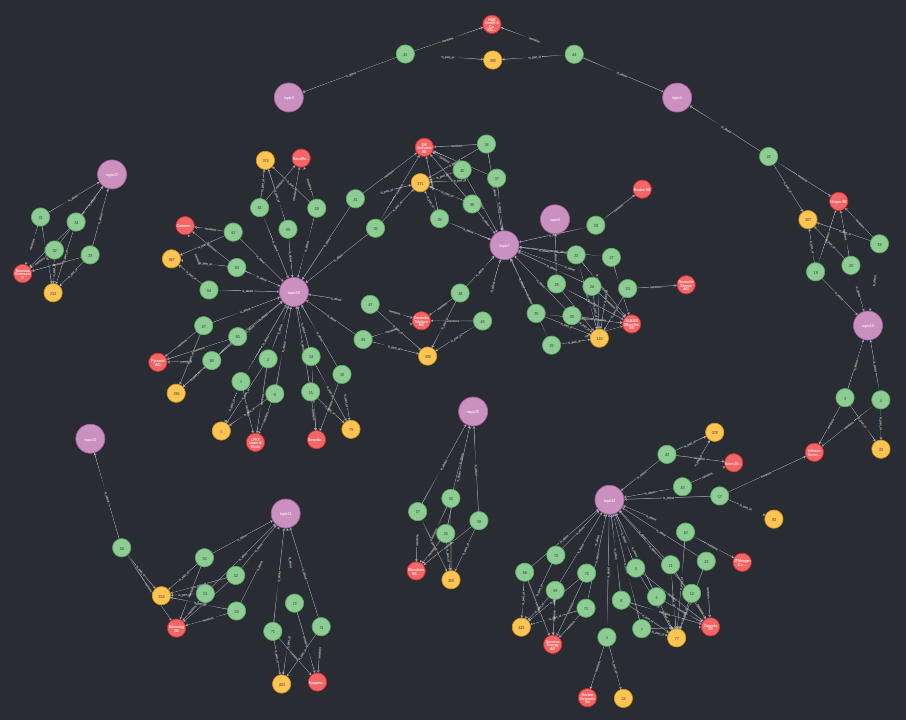
\includegraphics[width=1.0\textwidth]{Assets/kg-data-1}
    \caption{Knowledge Graph after Data Loading}
    \label{fig:kg-data-1}
\end{figure}

Zooming into an exemplary and disconnected Sub-Graph reveals some Relationships and Node properties, see Figure \ref{fig:kg-data-2}:

\begin{figure}[H]   %[h] puts picture right here. 't' stands for to, 'b' stands for bottom
    \centering
    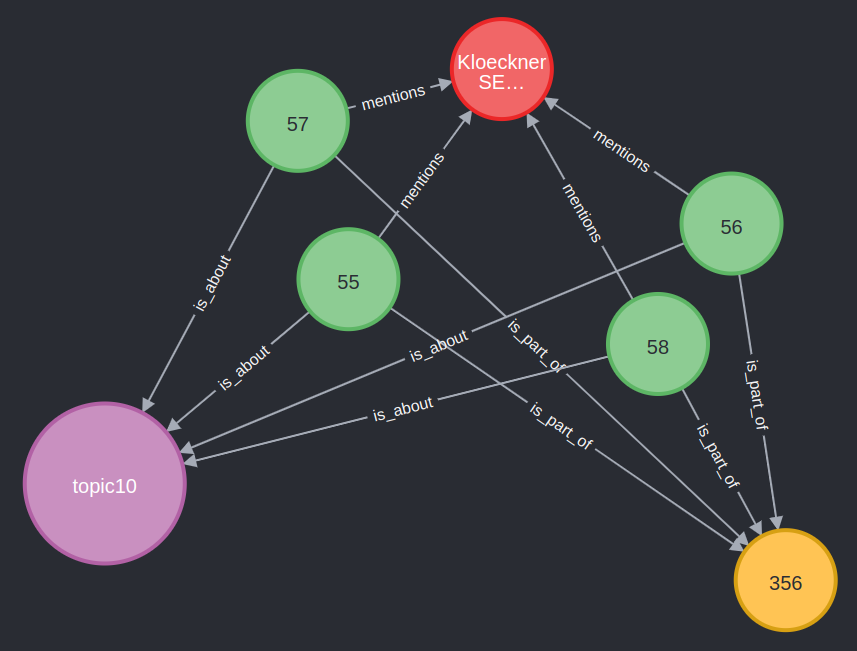
\includegraphics[width=1.0\textwidth]{Assets/kg-data-2}
    \caption{Exemplary, Disconnected Sub-Graph}
    \label{fig:kg-data-2}
\end{figure}

In the Sub-Graph (Fig.\ref{fig:kg-data-2}), a pink \emph{Topic} Node with its \emph{top\_id},
four green \emph{Sentence} Nodes with their \emph{sent\_id},
a yellow \emph{Article} Node with its \emph{art\_id} and
a red \emph{Company} Node with its \emph{comp\_name} properties are displayed.

The information for each Node can be displayed individually once they are selected in the browser:

\begin{figure}[H]
        \centering
        \begin{subfigure}[b]{0.475\textwidth}
            \centering
            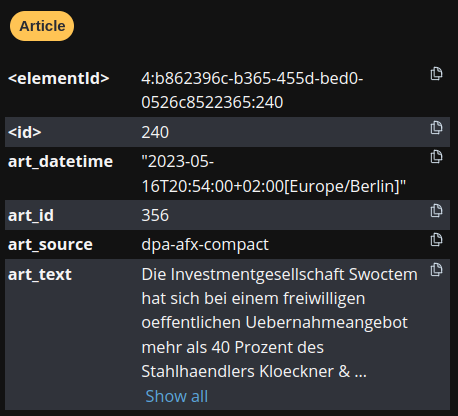
\includegraphics[width=\textwidth]{Assets/kg-data-3-article}
            \caption{\small Article}
            \label{fig:kg-data-3-article}
        \end{subfigure}
        \hfill
        \begin{subfigure}[b]{0.475\textwidth}
            \centering
            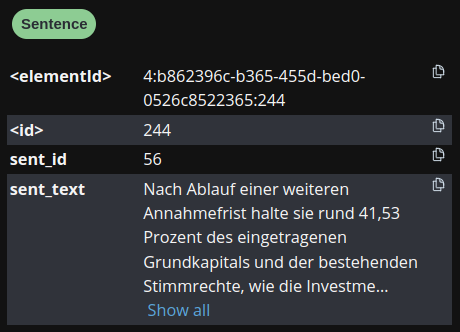
\includegraphics[width=\textwidth]{Assets/kg-data-3-sentence}
            \caption{\small Sentence}
            \label{fig:kg-data-3-sentence}
        \end{subfigure}
        \vskip\baselineskip
        \begin{subfigure}[b]{0.475\textwidth}
            \centering
            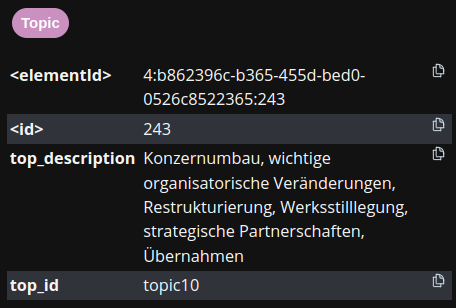
\includegraphics[width=\textwidth]{Assets/kg-data-3-topic}
            \caption{\small Topic}
            \label{fig:kg-data-3-topic}
        \end{subfigure}
        \hfill
        \begin{subfigure}[b]{0.475\textwidth}
            \centering
            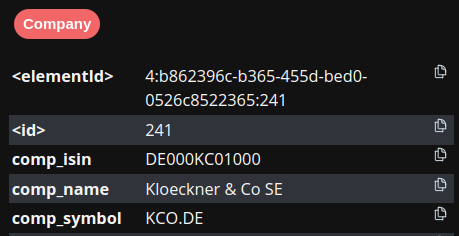
\includegraphics[width=\textwidth]{Assets/kg-data-3-company}
            \caption{\small Company}
            \label{fig:kg-data-3-company}
        \end{subfigure}
        \caption{\small neo4j: Nodes and their Properties}
        \label{fig:nodes-and-props}
\end{figure}

The four boxes in Figure \ref{fig:nodes-and-props} show the Node properties for the respective \emph{Nodes} that were previously loaded.

\section{External Data}
Publicly accessible triple stores \cite{triple-store}, such as DBPedia \cite{dbpedia} or WikiData \cite{wikidata}, can be used to enrich the Knowledge Graph with external data.
For external data to be added to the existing Knowledge Graph, a unique and common identifier that exists in these triple stores, is necessary.
The previously discussed \gls{isin}, that was mapped from the Company Symbol (see Section \ref{par:symbol-isin}), is such an identifier.
The \emph{import\_wikidata\_id()} function in Python-Code \ref{code:import-wikidata-id} uses the \gls{isin} to retrieve the \emph{Wikidata entity id} \cite{wiki-entity-id} for each of the companies in the Knowledge Graph.

\begin{listing}[H]
    \captionof{listing}{Function: import\_wikidata\_id()}
    \inputminted[
    firstline=84,
    lastline=114,
    firstnumber=84,
    ]{python}{/media/rainergo/PROJECTS/UASFRA-MS-Thesis/src/F_knowledge_graph/B_graph_construction.py}
    \label{code:import-wikidata-id}
\end{listing}

\paragraph{SPARQL}
The function in lines 94-98 embeds a SPARQL \cite{sparql} query that is sent via an http-request to the Wikidata Query Service with the URL
\begin{center}
\emph{https://query.wikidata.org/sparql}
\end{center}
referenced in line 101.
SPARQL is a query language to query and retrieve stored RDF data such as Wikidata or DBPedia entities \cite{sparql}.
Wikidata and DBPedia are considered publicly available triple stores \cite{triple-store}.\\
neo4j's apoc \cite{neo4j-apoc} library processes the SPARQL response (lines 106-109) and inserts the \emph{wikidataID} into the respective property of each \emph{Company} Node, if the Wikidata entity page contains this information.\\

There are two other functions that can enrich the Knowledge Graph via SPARQL queries, namely
\emph{import\_data\_from\_wikidata()} and \emph{import\_data\_from\_dbpedia()}
in the \emph{GraphConstruction} class.
They can load any available information from triple stores that have a link to a \emph{Wikidata entity id} \cite{wiki-entity-id} or \gls{isin}.\\
To show some examples, I have used these functions to load the \emph{Industry} category, the home \emph{Country} and a short \emph{Abstract} about the companies
from Wikidata and DBPedia.
The respective SPARQL queries, that are automatically generated by the two functions, for demonstration purposes were manually composed and are shown in Figure \ref{fig:sparql-requests}.

\begin{figure}[H]
        \centering
        \begin{subfigure}[b]{0.80\textwidth}
            \centering
            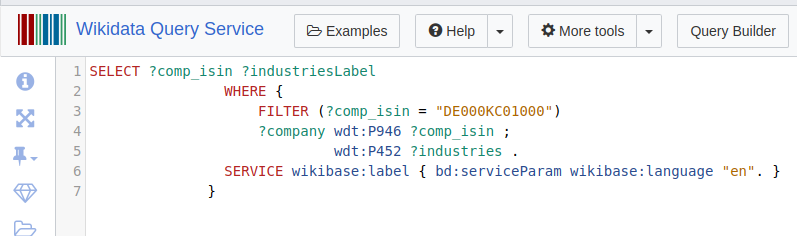
\includegraphics[width=\textwidth]{Assets/wikirequest-indu}
            \caption{\small P452 - Industry}
            \label{fig:wikirequest-indu}
        \end{subfigure}
        \vskip\baselineskip
        \begin{subfigure}[b]{0.80\textwidth}
            \centering
            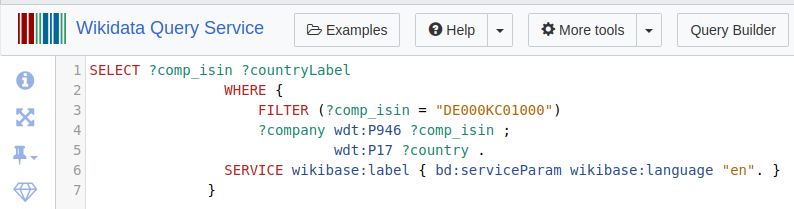
\includegraphics[width=\textwidth]{Assets/wikirequest-country}
            \caption{\small P17 - Country}
            \label{fig:wikirequest-country}
        \end{subfigure}
        \vskip\baselineskip
        \begin{subfigure}[b]{0.55\textwidth}
            \centering
            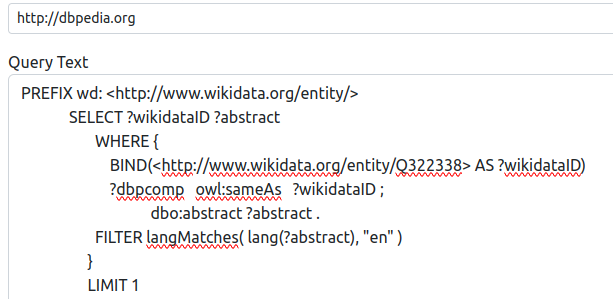
\includegraphics[width=\textwidth]{Assets/dbpedia-request-abstract}
            \caption{\small dbo:abstract - Abstract}
            \label{fig:dbpedia-request-abstract}
        \end{subfigure}
        \caption{\small SPARQL: Queries to enrich Knowledge Graph}
        \label{fig:sparql-requests}
\end{figure}

In the neo4j Subgraph \ref{fig:kg-data-4-company}, the \emph{Company} Node properties for \emph{Kloeckner \& Co SE} now include the information
for \emph{Industry}, \emph{Country} and an \emph{Abstract}.

\begin{figure}[H]
	\centering
	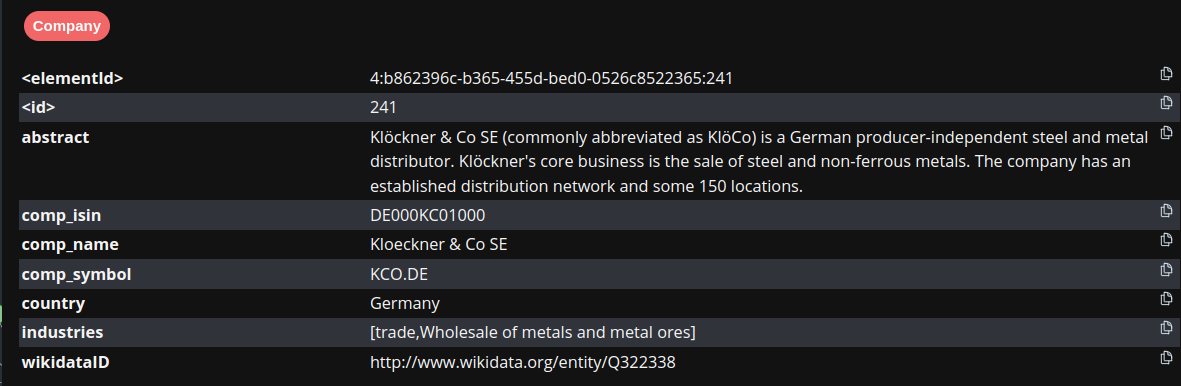
\includegraphics[width=\textwidth]{Assets/kg-data-4-company}
	\caption{Company Node after Data Enrichment}
	\label{fig:kg-data-4-company}
\end{figure}


\section{Information Retrieval}
With the data from the DataFrame and from external sources loaded, the Knowledge Graph can now be queried to retrieve information.

\paragraph{\gls{cypher} Queries}
\gls{cypher} queries provide a visual way to reveal patterns and relationships by using a human-friendly ASCII-based type of syntax \cite{neo4j}.

\begin{center}
    \textbf{(:nodes) - [:ARE\_CONNECTED\_TO] → (:otherNodes)}
\end{center}

Round brackets are used to represent \emph{(:Nodes)}, and \emph{-[:ARROWS]→} to represent a relationship between the \emph{(:Nodes)}.
\gls{cypher} queries can be used to reveal a wide range of Knowledge Graph information ranging from simple property values to complex, multi-hop relations.\\
A user, for instance, could be interested in news articles about a particular company such as \emph{Brenntag SE} or all companies that are mentioned in sentences about \emph{Topic12} on a specific day and so would compose the following Cyper queries:

\begin{figure}[H]
        \centering
        \begin{subfigure}[b]{\textwidth}
            \centering
            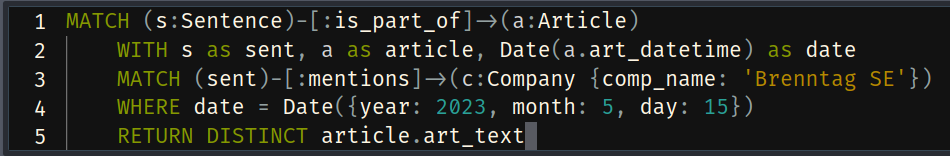
\includegraphics[width=\textwidth]{Assets/cypher-1}
            \caption{\small Cypher Query 1: Articles about \emph{Brenntag SE}}
            \label{fig:cypher-1}
        \end{subfigure}
        \vskip\baselineskip
        \begin{subfigure}[b]{\textwidth}
            \centering
            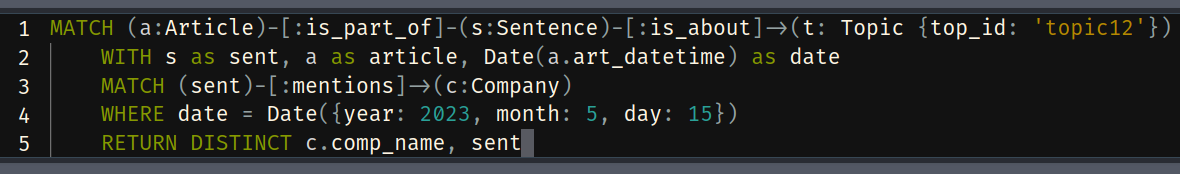
\includegraphics[width=\textwidth]{Assets/cypher-2}
            \caption{\small Cypher Query 2: Companies, Sentences about \emph{Topic12}}
            \label{fig:cypher-2}
        \end{subfigure}
        \caption{\small Cypher Queries 1-2}
        \label{fig:cypher-queries-pair1}
\end{figure}

Another user could be interested only in certain industry news for a particular day or only in sentences with certain topics and about companies that are located in Germany.
He could compile these \gls{cypher} queries:

\begin{figure}[H]
        \centering
        \begin{subfigure}[b]{\textwidth}
            \centering
            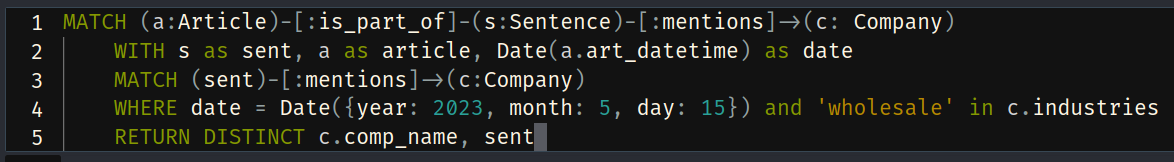
\includegraphics[width=\textwidth]{Assets/cypher-3}
            \caption{\small Cypher Query 3: Sentences about Industry \emph{Wholesale}}
            \label{fig:cypher-3}
        \end{subfigure}
        \vskip\baselineskip
        \begin{subfigure}[b]{\textwidth}
            \centering
            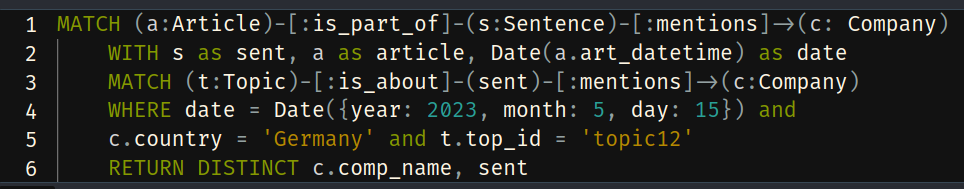
\includegraphics[width=\textwidth]{Assets/cypher-4}
            \caption{\small Cypher Query 4: German Companies, Sentences about Topic12}
            \label{fig:cypher-4}
        \end{subfigure}
        \caption{\small Cypher Queries 3-4}
        \label{fig:cypher-queries-pair2}
\end{figure}

The queries could be even more specific and nested and so reveal deep interrelations between \emph{Companies}, \emph{Articles}, \emph{Topics} and \emph{Sentences} and their particular properties.
The queries can be executed via the Python plugin or directly in the browser console and will be returned either as Graph visualization or as String in \gls{json} format.

\section{Sentence Embeddings and Sentiment}
So far, the \emph{Sentence} information is only stored as text in the Node's property \emph{sent\_text}.
But the \emph{Embedder} class in the \emph{F\_knowledge\_graph} directory allows to contextually embed (see Section \ref{subsec:contextual-word-embeddings}) these sentences.

The method \emph{create\_text\_embedding()} (Python-Code \ref{code:sent-text-embed}) in the previously cited \emph{GraphConstruction} class conveniently embeds all the sentences in the Knowledge Graph and
stores the embedding vector of size 768 in the new \emph{Sentence} Node property \emph{sent\_text\_embedding}:

\begin{listing}[H]
    \captionof{listing}{Function: create\_text\_embedding()}
    \inputminted[
    firstline=201,
    lastline=227,
    firstnumber=201,
    ]{python}{/media/rainergo/PROJECTS/UASFRA-MS-Thesis/src/F_knowledge_graph/B_graph_construction.py}
    \label{code:sent-text-embed}
\end{listing}
Once the function has run, each \emph{Sentence} text has been embedded and added to the \emph{Sentence} properties.
It again can be shown in the browser by selecting the respective \emph{Sentence} Node:

\begin{figure}[H]   %[h] puts picture right here. 't' stands for to, 'b' stands for bottom
    \centering
    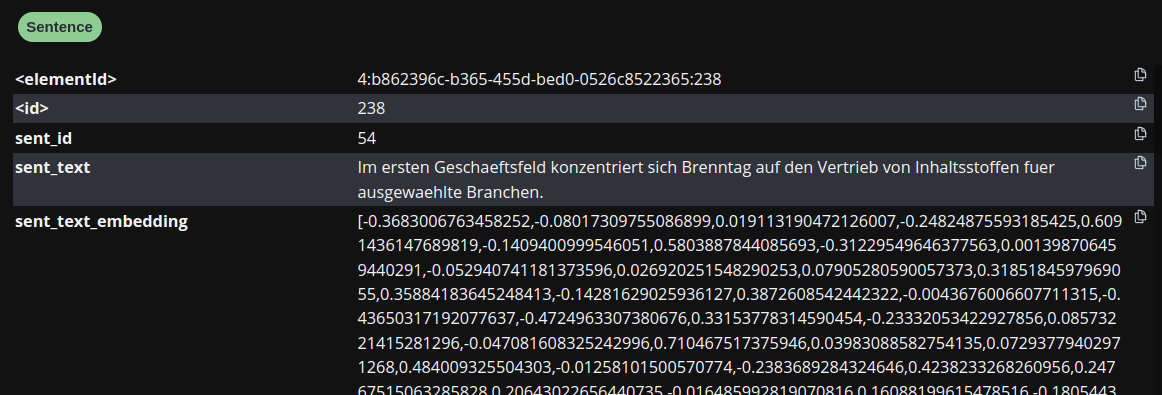
\includegraphics[width=\textwidth]{Assets/sent-embed}
    \caption{BERT Sentence Embedding}
    \label{fig:sent-embed}
\end{figure}
As here a \gls{BERT} (\emph{bert-base-uncased}) model was used for the embeddings, the dimension of the embedding vector is 768.\\

With such sentence embeddings, it is possible to train a \emph{Sentiment Model} to classify these sentences into different categories.
For instance, a \emph{Sentiment Model} could be trained with three classes such as:

\begin{itemize}
    \item POSITIVE
    \item NEUTRAL
    \item NEGATIVE
\end{itemize}

Afterward, this model can predict the sentiment of all sentences based on their embeddings, and the respective \emph{Sentiment Class} would be added to the \emph{Sentence} Node properties.
\gls{cypher} queries could then retrieve and filter sentences with a certain sentiment.\\
A user who wanted to see
\begin{center}
\emph{"only NEGATIVE news sentences about German companies"}
\end{center}
could run the following exemplary \gls{cypher} query:

\begin{figure}[H]   %[h] puts picture right here. 't' stands for to, 'b' stands for bottom
    \centering
    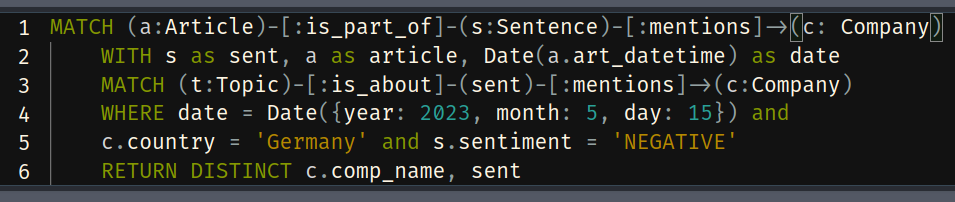
\includegraphics[width=\textwidth]{Assets/sentiment}
    \caption{Sentence: Sentiment Classification}
    \label{fig:sentiment}
\end{figure}
Every such data enrichment of the Knowledge Graph, here the enrichment with sentence embeddings and sentiment classes, can enhance the Knowledge Graph's capability to retrieve complex information.

\section{\gls{graph-bot}}
The query language \gls{cypher} is relatively easy to learn and user-friendly, but not as friendly as the human language itself.\\
neo4j \cite{neo4j} via the LangChain \cite{LangChain} library offers a \emph{GraphCypherQAChain} and \emph{Neo4jGraph} module.
These modules, together with other LangChain components (see Section \ref{subsec:langchain-explain}), can be used to create a ChatBot that converts human language to \gls{cypher} queries, and \gls{cypher} responses back to human language.
This was done in the \emph{D\_graph\_bot.py} (Python-Codes \ref{code:chatbot-1} to \ref{code:chatbot-4}) module in the \emph{F\_knowledge\_graph} directory.

\begin{listing}[H]
    \captionof{listing}{Knowledge Graph Chatbot: init}
    \inputminted[
    firstline=70,
    lastline=82,
    firstnumber=70
    ]{python}{/media/rainergo/PROJECTS/UASFRA-MS-Thesis/src/F_knowledge_graph/D_graph_bot.py}
    \label{code:chatbot-1}
\end{listing}

The LangChain pipeline or chain uses an \gls{llm} (line 84 of Python-Code \ref{code:chatbot-1}) and explanatory Examples of which some are
shown in Python-Code \ref{code:chatbot-2}:

\begin{listing}[H]
    \captionof{listing}{Knowledge Graph Chatbot: Examples}
    \inputminted[
    firstline=14,
    lastline=35,
    firstnumber=14,
    fontsize=\tiny,
    ]{python}{/media/rainergo/PROJECTS/UASFRA-MS-Thesis/src/F_knowledge_graph/D_graph_bot.py}
    \label{code:chatbot-2}
\end{listing}
\begin{listing}[H]
    \captionof{listing}{Knowledge Graph Chatbot: \gls{prompt}}
    \inputminted[
    firstline=92,
    lastline=114,
    firstnumber=92,
     fontsize=\tiny,
    ]{python}{/media/rainergo/PROJECTS/UASFRA-MS-Thesis/src/F_knowledge_graph/D_graph_bot.py}
    \label{code:chatbot-3}
\end{listing}

These examples are then embedded into a \gls{prompt} (Python-Code \ref{code:chatbot-3}) which,
along the \emph{User Question}, is sent to the \gls{llm}, see Python-Code \ref{code:chatbot-4}:

\begin{listing}[H]
    \captionof{listing}{Knowledge Graph Chatbot: Request to \gls{llm}}
    \inputminted[
    firstline=122,
    lastline=131,
    firstnumber=122
    ]{python}{/media/rainergo/PROJECTS/UASFRA-MS-Thesis/src/F_knowledge_graph/D_graph_bot.py}
    \label{code:chatbot-4}
\end{listing}

An exemplary user that is interested in
\begin{center}
\emph{companies that were mentioned in sentences published between certain dates}
\end{center}
could pose text questions to the \gls{graph-bot} as shown in Python-Code \ref{code:chatbot-5}:

\begin{listing}[H]
    \captionof{listing}{\gls{graph-bot}: User Question}
    \inputminted[
    firstline=135,
    lastline=140,
    firstnumber=135
    ]{python}{/media/rainergo/PROJECTS/UASFRA-MS-Thesis/src/F_knowledge_graph/D_graph_bot.py}
    \label{code:chatbot-5}
\end{listing}

If the parameter \emph{verbose} (line 124 in Python-Code \ref{code:chatbot-4}) is set to \emph{True},
the \gls{graph-bot}'s processing steps will be displayed as depicted in Figures \ref{fig:chatbot-1} to \ref{fig:chatbot-3}:

\begin{figure}[H]   %[h] puts picture right here. 't' stands for to, 'b' stands for bottom
    \centering
    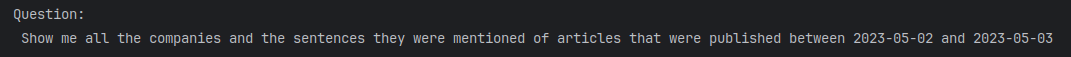
\includegraphics[width=\textwidth]{Assets/chatbot-question}
    \caption{\gls{graph-bot} - Part 1: Question}
    \label{fig:chatbot-1}
\end{figure}

After the user has sent his question to the \gls{graph-bot} (Fig. \ref{fig:chatbot-1}) ...
\begin{figure}[H]   %[h] puts picture right here. 't' stands for to, 'b' stands for bottom
    \centering
    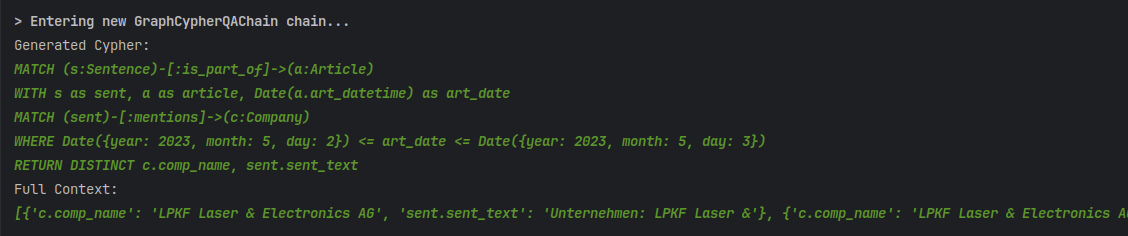
\includegraphics[width=\textwidth]{Assets/chatbot-processing}
    \caption{\gls{graph-bot} - Part 2: Creating \gls{cypher} Queries}
    \label{fig:chatbot-2}
\end{figure}
... the \gls{graph-bot} converts this question into a corresponding \gls{cypher} query (Figure \ref{fig:chatbot-2}) and sends it to the neo4j graph database.

\begin{figure}[H]   %[h] puts picture right here. 't' stands for to, 'b' stands for bottom
    \centering
    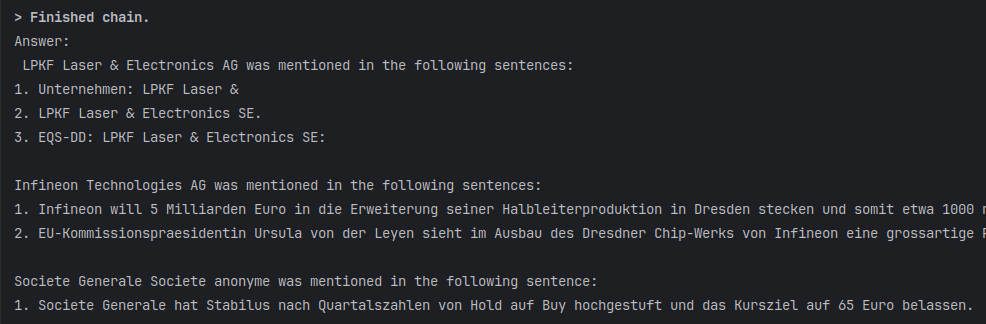
\includegraphics[width=\textwidth]{Assets/chatbot-answer}
    \caption{\gls{graph-bot} - Part 3: Answer}
    \label{fig:chatbot-3}
\end{figure}

The JSON object returned by the neo4j graph database is then converted to human-readable text (Figure \ref{fig:chatbot-3}) and returned to the user.

\paragraph{\gls{graph-bot} vs. \gls{llm} Chatbot}
The \gls{graph-bot} is comparable to an \gls{llm} ChatBot such as ChatGPT in that a user can ask questions or \gls{prompt} the \gls{llm} ChatBot for specific tasks.
But they differ in that the \gls{graph-bot}'s answer is based on concrete text and factual data in news articles whereas the \gls{llm} ChatBot relies
on next-word probabilities.
Whereas the \gls{graph-bot} often returns the literal text of the existing news article in its answer (see Figure \ref{fig:chatbot-3}),
the \gls{llm} ChatBot returns newly generated text that might be contextually correct, but is often factually incorrect.

This lies in the nature of \gls{llm}s as they are trained to generalize well, but not to memorize the data they were trained with (as discussed in Section \ref{par:hallucination}).

Checking and validating the returned text from the \gls{llm} ChatBot is tedious and cumbersome,
whereas for the GraphBot, this can easily be done with \gls{cypher} queries.\\
In this sense, the \gls{graph-bot} is superior to a general \gls{llm} ChatBot if the user expects actual facts instead of newly generated text.


\paragraph{Production Use Case}
The \gls{graph-bot} currently only uses a few examples in its \gls{prompt} which are probably not enough to constantly get satisfactory
and correct answers.
For a production use case, the provided examples would need some enhancement and refinement.\\
Apart from this, the \gls{graph-bot} is a useful human interaction tool for users that do not want to write \gls{cypher} queries,
but use human language to retrieve information from the Knowledge Graph.


\paragraph{Knowledge Graph as RAG}
The Knowledge Graph served the \gls{graph-bot} as a data retriever and thus can be considered a \gls{RAG} system (see Section \ref{par:rag-systems}).
While typical RAG systems might distinguish documents with strongly different context, they usually suffer from the following shortcomings \cite{rag-cririque}:

\begin{itemize}
    \item Misunderstanding of documents that contain nuanced context differences.
    \item Chunking of document breaks its context.
    \item Vector database contains irrelevant information.
\end{itemize}

These issues are addressed by the Knowledge Graph in this project:
The \gls{gen-llm} in the Coreference Resolution and Topic Modelling pipeline could also semantically misunderstand the news article sentences,
but this is less likely as both pipeline components are tightly defined and accompanied by dedicated \gls{prompt} examples.
It was shown in the Topic Modelling section (see Section \ref{sec:topic-gen-llm}) that the \gls{gen-llm} component can indeed distinguish nuanced differences in context.
The relevant sentences are much shorter, more focused and less generic than typical documents in a vector database.
Both, the chunking and semantic interpretation is done on the sentence level so that the chunking cannot split the sentence's context \footnote{Under the assumption that sentence splitting works correctly}.
Each sentence with a found company is all relevant and thus cannot contain irrelevant information.\\
Thus, the vector database could be replaced by such a Knowledge Graph.
This is also supported by a recent research paper from Microsoft: GraphRAG \cite{graphrag}.
Instead of feeding the news article text to a vector database, it could be extracted and inserted into a Knowledge Graph, as it was shown in this project.



